%------------------------------------------------------------------------------
% No implementation, software engineering details, or project management
%------------------------------------------------------------------------------

%------------------------------------------------------------------------------

\begin{subsection}{The Elevator Pitch}
  Whilst advances in technology have revolutionised other industries and parts of agriculture, bringing with it radically improved methods and cost efficiencies, the way in which we identify and mark cattle is practically archaic.
  
  Globally, and particularly in developing countries, cattle are revered. It is in these countries where, most frequently, cattle are the least protected from theft, with each cow often representing a high percentage of a farmer's livelihood and wealth.
  
  CowHub provides a database of cattle and identifies cattle without the need for physical deformation. In doing so, any cattle that has not been tampered with can be identified as belonging to it's owner deterministically and with near certain reliability.
\end{subsection}
 
%------------------------------------------------------------------------------

\begin{subsection}{Project Description}
  This project will focus on providing a technology-based answer to this problem by providing a user-friendly platform, alleviating all associated pain for cattle, whilst offering benefits that only a scalable, centralised system is able to offer, as above.
    
  There are three key objectives for this project:
  
  \begin{itemize}
  	\item To offer a \textbf{harmless, physically non-destructive alternative} to current methods used to identify cattle
  	\item Provide a service that \textbf{allows the identification of cattle}
  	\item Collect data on cattle from farmers to be able to \textbf{build and use a widespread catalogue of information regarding cattle and their movements}
  \end{itemize}
\end{subsection}

%------------------------------------------------------------------------------

\begin{subsection}{What is the need for the project?}
  The process of marking cattle can be incredibly painful, regardless of the age of the cattle. Clearly, being subject to this pain, and the witnessing of the pain of a calf by a mother, is a point of controversy for animal rights activists. Members of the public feel so strongly about the issue that they have protested by branding themselves in public, much to the disgust of onlookers~\cite{theguardian1}. 
  
  Whilst branding itself is no longer carried out in the United Kingdom, current methods, including piercing a cattle's ears, are still in use today and are without animal-friendly competition currently. 

  \begin{figure}[H]
  	\centering
    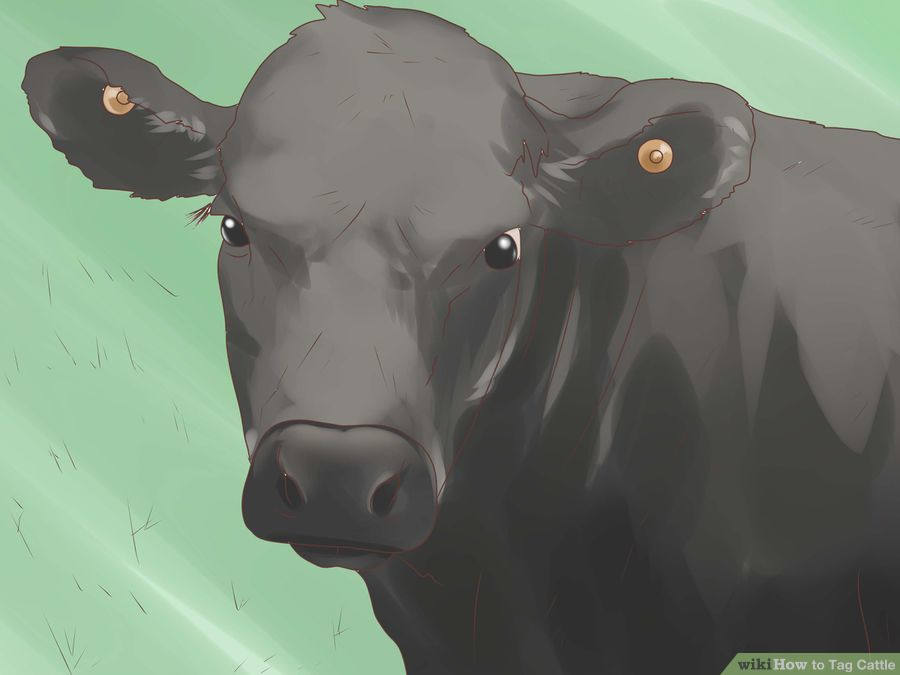
\includegraphics[width=0.5\textwidth]{images/cattle-with-ear-tag.jpg}
  	\caption[Cattle ear tagging]{
      Illustration of a cattle's head, demonstrating the position and rough size of cattle tags from the front. \cite{wikihow1}
  	}
  \end{figure}
  
  CowHub provides a user friendly platform to easily register and manage the information of a cattle without the pain-inflicting measures of the current system.

\end{subsection}
